\subsection{Uneigentliche Integrale}
\begin{bsp}
	{Zwei typische Fragestellungen}{}
	Der Graph der Funktion $f(x) = \frac{1}{x}, \, x \in [1, \infty[$ erstreckt sich ins Unendliche. Im Folgenden untersuchen wir einerseits den Flächeninhalt $A$ des Gebietes $G$ zwischen dem Graphen von $f$ und der $x$-Achse und andererseits den Rauminhalt $V$ des Körpers, der durch Rotation von $G$ um die $x$-Achse entsteht.
	\begin{enumerate}
		\item Bestimme $A(t) = \int_1^t f(x) dx$ und $V(t) = \pi \int_1^t (f(x))^2 dx$ für $t\in [1, \infty[$
		\item Bestimme $\lim_{t\to\infty} A(t)$ und $\lim_{t\to\infty} V(t)$, falls die Grenzwerte existieren.
	\end{enumerate}
\end{bsp}
\clearpage
\begin{definition}
	{Uneigentliche Integrale}{}
	\begin{center}
		
\includegraphics[width = \textwidth]{media/defUneigentlicheIntegrale.png}
	\end{center}
\end{definition}
\begin{bsp}
	{Ein uneigentliches Integral}{}
	\begin{align*}
		\int_{4}^{\infty} \frac{4-x}{x^3} \,dx & = \lim_{{t \to \infty}} \int_{4}^{t} \frac{4-x}{x^3} \,dx                                      \\
		                                       & = \lim_{{t \to \infty}} \int_{4}^{t} \left( \frac{4}{x^3} - \frac{1}{x^2} \right) \,dx         \\
		                                       & = \lim_{{t \to \infty}} \int_{4}^{t} \left( 4\cdot x^{-3} - x^{-2} \right) \,dx                \\
		                                       & = \lim_{{t \to \infty}} \left[ 4\cdot \left(-\frac{1}{2}\right)x^{-2} + x^{-1} \right]_{4}^{t} \\
		                                       & = \lim_{{t \to \infty}} \left( -2t^{-2} + t^{-1} - (-2 \cdot 4^{-2} + 4^{-1}) \right)          \\
		                                       & = 0 + 0 - \left( -\frac{1}{8} + \frac{1}{4} \right)                                            \\
		                                       & = -\frac{1}{8}
	\end{align*}
	\begin{center}
		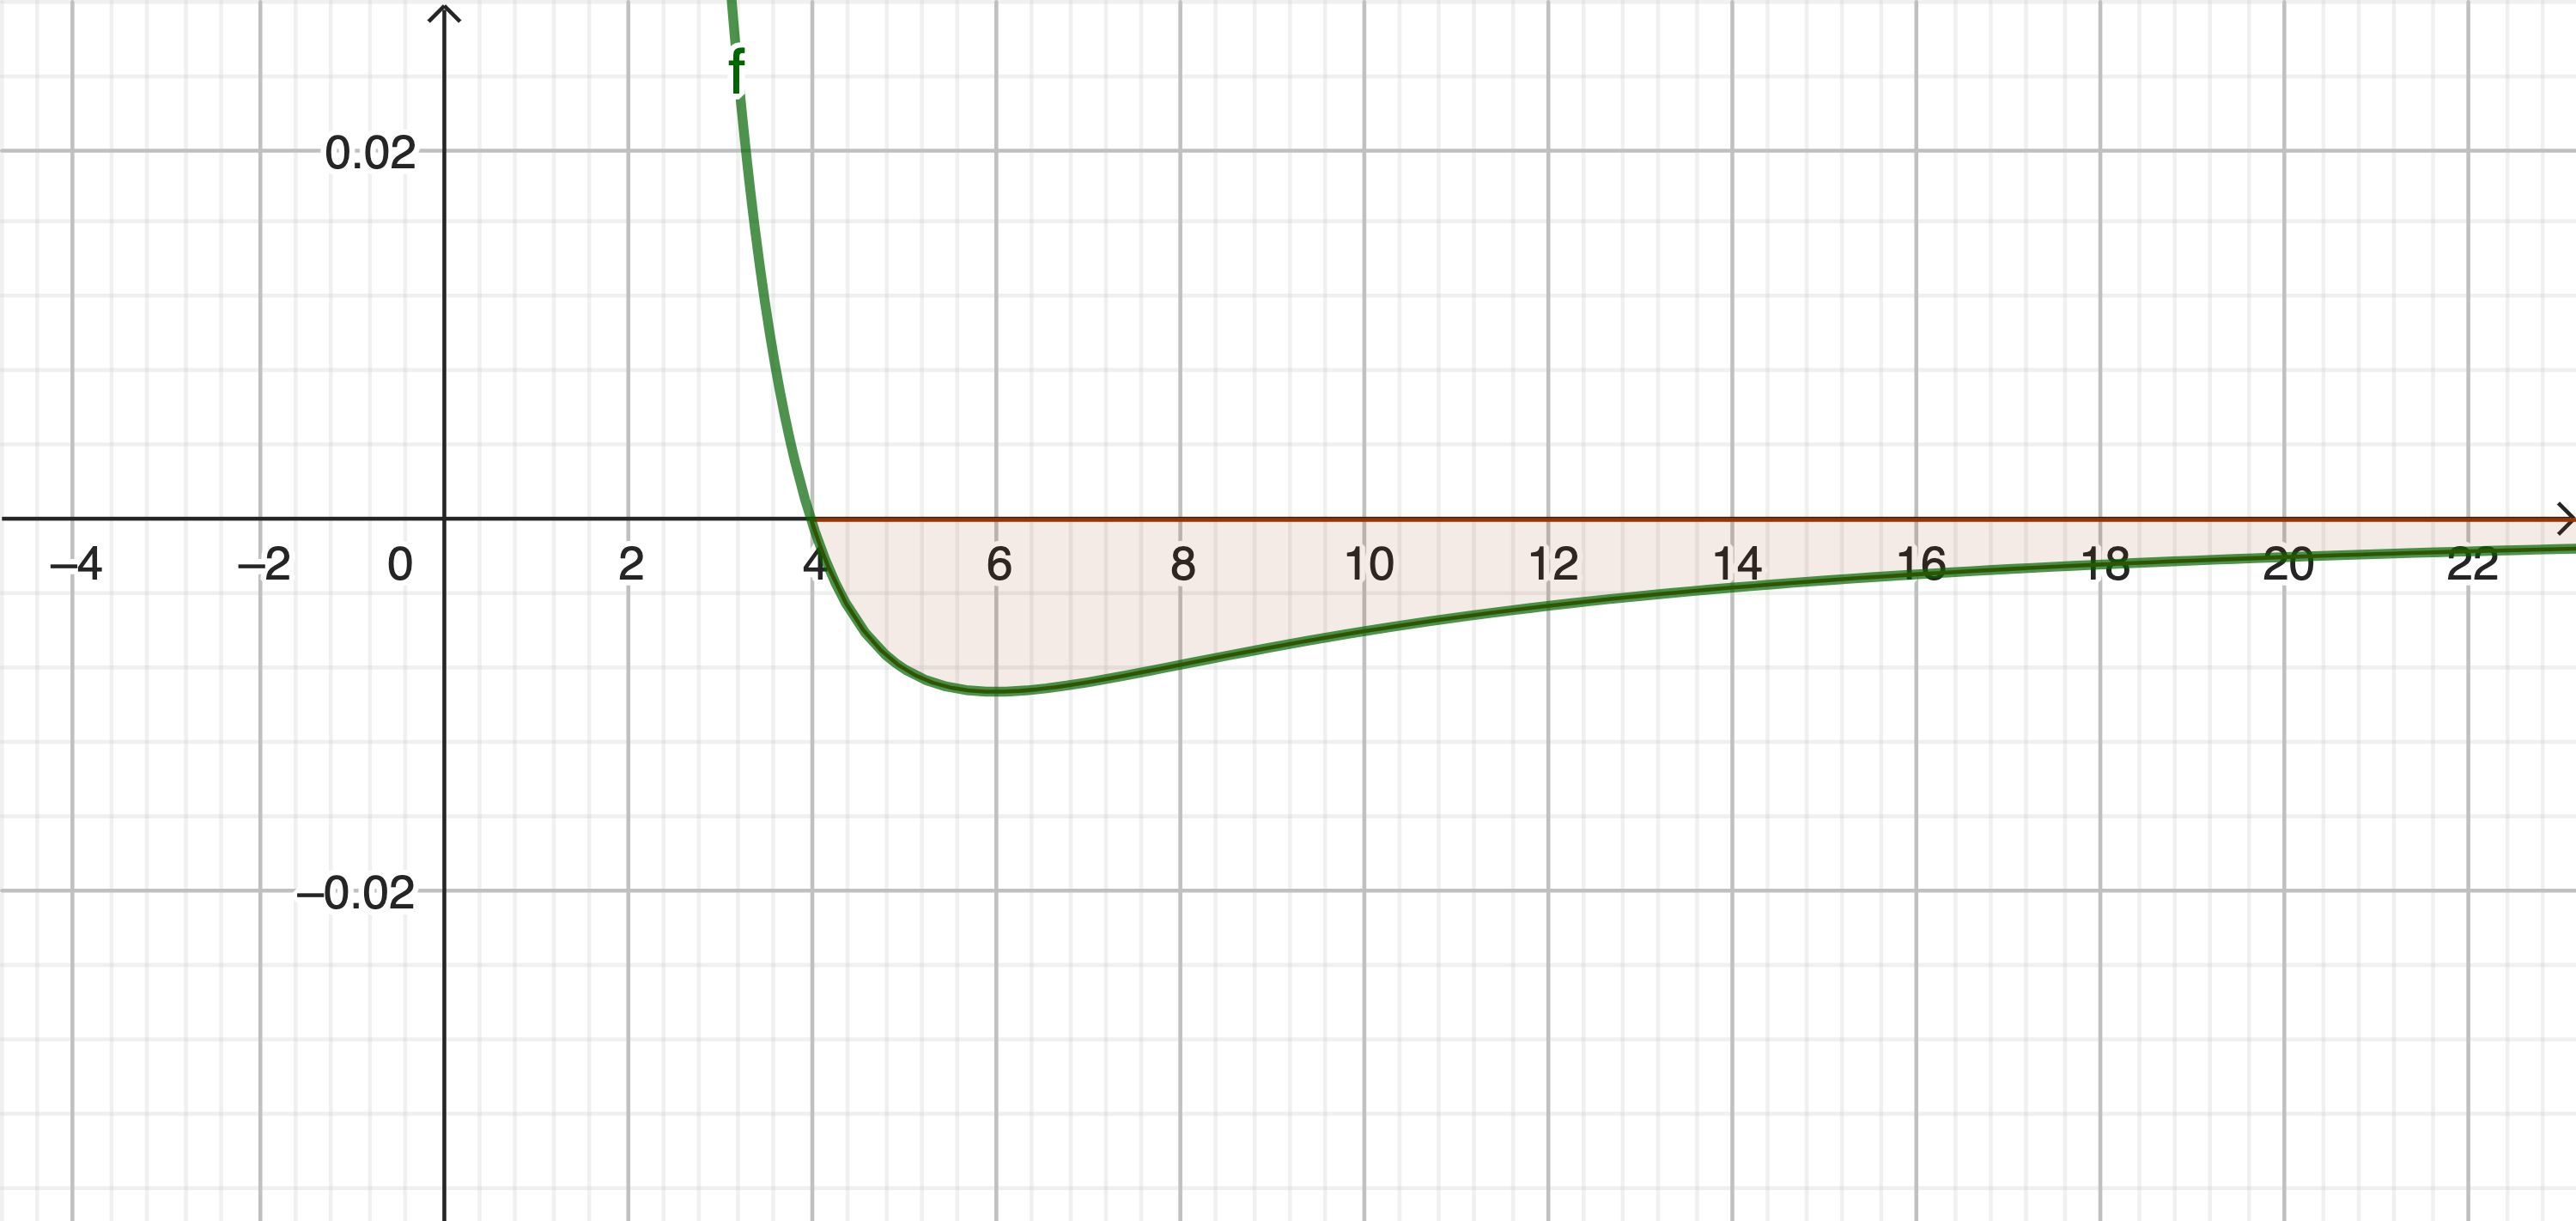
\includegraphics[width = 0.5 \textwidth]{media/bspUneigentlich.png}
	\end{center}
\end{bsp}
\clearpage
\begin{bsp}
	{Ein uneigentliches Integral mit linearer Substitution}{}
	$$\int_{3}^{\infty} \frac{1}{(2x+1)^2} dx = ?$$
	Die Stammfunktion lässt sich mit linearer Substitution finden: $$\int \frac{1}{(2x+1)^2} dx= \int (2x+1) ^{-2} dx= -(2x+1)^{-1}\cdot \frac{1}{2} + C$$
	Damit folgt:
	\begin{align*}
		\int_{3}^{\infty} \frac{1}{(2x+1)^2} dx & = \lim_{t \to \infty}  \int_{3}^{t} (2x+1) ^{-2} dx                                         \\
		                                        & = \lim_{t \to \infty} \left[-(2x+1)^{-1}\cdot \frac{1}{2}\right]_3^t                        \\
		                                        & = \lim_{t \to \infty} \left(-\frac{1}{(2t+1)\cdot 2} + \frac{1}{(2\cdot 3+1)\cdot 2}\right) \\
		                                        & = \frac{1}{14}
	\end{align*}
	\begin{center}
		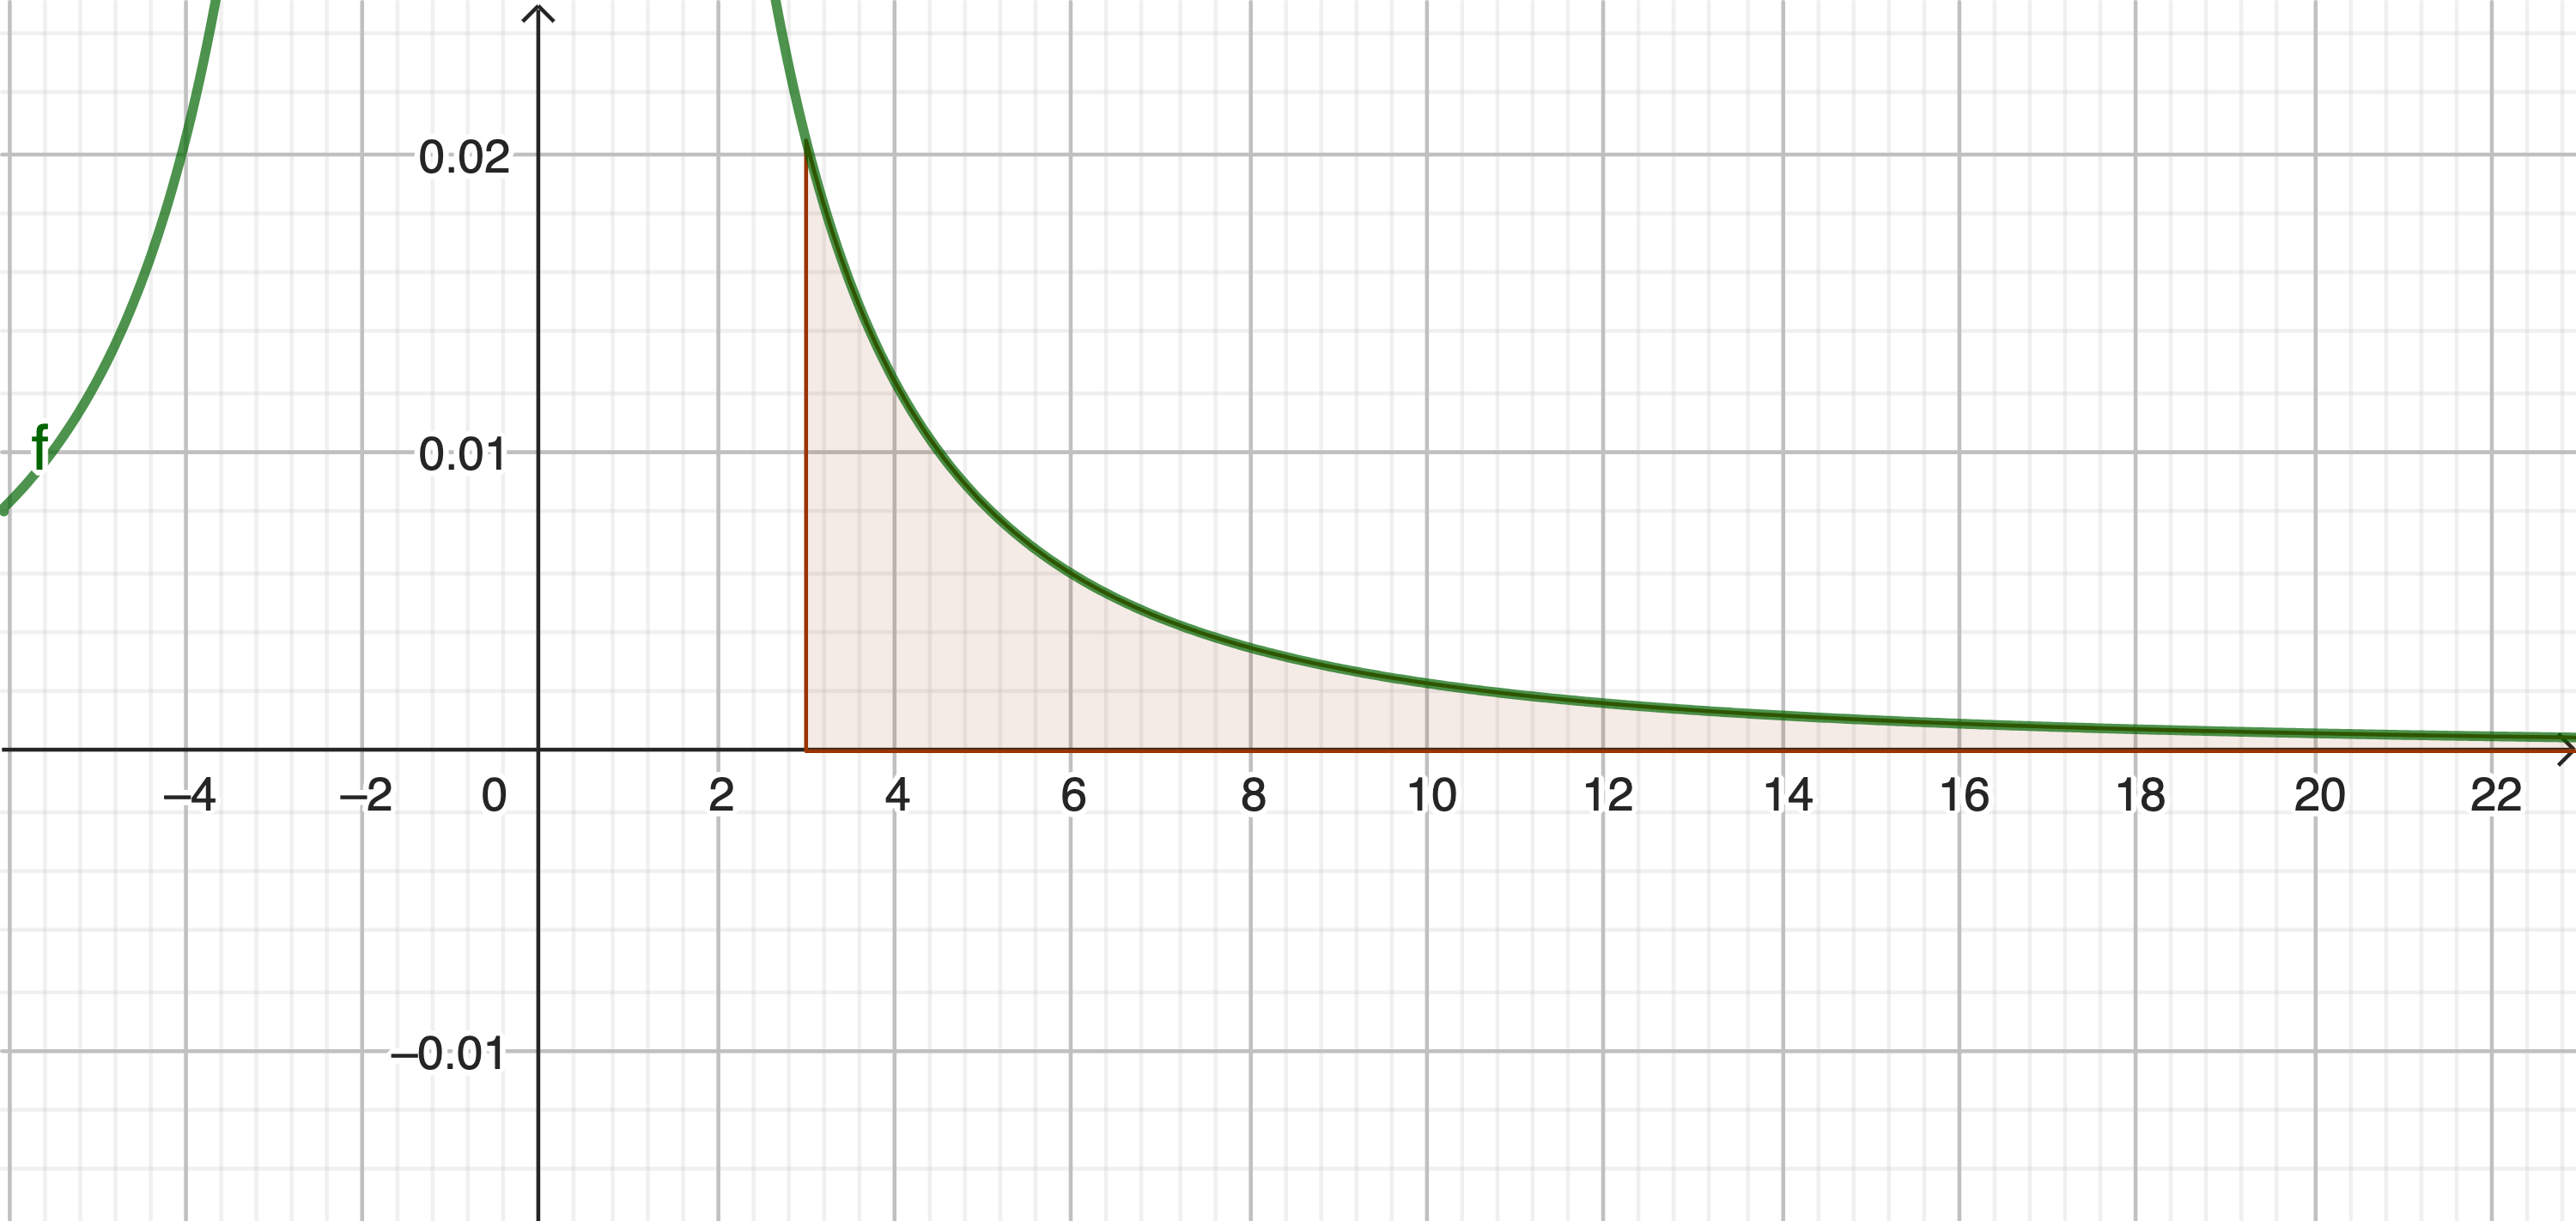
\includegraphics[width = 0.5 \textwidth]{media/bspUneigentlich2.png}
	\end{center}
\end{bsp}
